\documentclass[11pt, aspectratio=169, UTF8, fontset=none]{ctexbeamer}

% 选择学术界常用的经典主题（底部自带作者、标题和页码导航）
\usetheme{Madrid}
\usepackage{booktabs}
\usepackage{amsmath}

% ==================== 首行缩进和段落间距设置 ====================
\setlength{\parindent}{0pt}
\setlength{\parskip}{0.5\baselineskip}

% ==================== 自定义底部导航栏 (三段式) ====================
\setbeamertemplate{navigation symbols}{}

\setbeamertemplate{footline}{
  \leavevmode%
  \hbox{%
  % 左侧：报告标题（占屏幕宽度的 40%）
  \begin{beamercolorbox}[wd=.4\paperwidth,ht=2.25ex,dp=1ex,left,leftskip=2ex]{author in head/foot}%
    \usebeamerfont{author in head/foot}\insertshorttitle
  \end{beamercolorbox}%
  % 中间：当前章节（占屏幕宽度的 40%）
  \begin{beamercolorbox}[wd=.4\paperwidth,ht=2.25ex,dp=1ex,center]{title in head/foot}%
    \usebeamerfont{title in head/foot}\insertsectionhead
  \end{beamercolorbox}%
  % 右侧：幻灯片进度（占屏幕宽度的 20%）
  \begin{beamercolorbox}[wd=.2\paperwidth,ht=2.25ex,dp=1ex,right,rightskip=2ex]{date in head/foot}%
    \usebeamerfont{date in head/foot}\insertframenumber{} / \inserttotalframenumber
  \end{beamercolorbox}}%
  \vskip0pt%
}

% ==================== 插图设置 ====================
\usepackage{graphicx}%图片宏包
\usepackage{subcaption}%子图宏包
%强制开启图表自动编号
\setbeamertemplate{caption}[numbered]
%将图表标签（“图”或“Figure”）的颜色强制改为黑色
\setbeamercolor{caption name}{fg=black}

% ==================== 代码框设置 ====================
\usepackage{listings}%代码高亮宏包
\usepackage{tcolorbox}%用于绘制带有背景色、圆角、边框的彩色盒子。
% 加载 tcolorbox 的官方扩展库，：
% 1. listings: 将底层的 listings 代码排版功能与 tcolorbox 结合，允许你在漂亮的盒子里直接渲染带语法高亮的代码(解锁 \begin{tcblisting} 环境)。
% 2. skins: 加载高级皮肤引擎(基于 TikZ)，解锁更多高级视觉效果，例如阴影、渐变色、无缝拼接以及更复杂的圆角/边框样式。
% 3. breakable: 允许分页。
\tcbuselibrary{listings, skins, breakable}

% 定义类似 GitHub 的浅灰色背景和边框颜色
\definecolor{codegray}{HTML}{F6F8FA}
\definecolor{framegray}{HTML}{D1D5DA}
\definecolor{keywordcolor}{HTML}{005CC5}
\definecolor{stringcolor}{HTML}{032F62}
\definecolor{commentcolor}{HTML}{6A737D}

\setmonofont{Consolas}%设置给代码环境用的等宽字体

% 定义一个新的环境：code
\newtcblisting{code}[1][]{
  listing only,
  breakable,
  colback=codegray,        % 背景色
  colframe=framegray,      % 边框色
  boxrule=1pt,             % 边框粗细
  arc=3pt,                 % 圆角大小
  outer arc=3pt,
  left=4pt, right=4pt, top=2pt, bottom=2pt, % 内部边距
  listing options={
	tabsize=4,               %告诉引擎1个Tab等于4个空格，消灭 ^^I
    columns=fullflexible,    %改用弹性对齐，防止引擎吞掉 \begin
    keepspaces=true,         %严格保留所有缩进
	mathescape=true,%允许注释使用latex公式
    basicstyle=\ttfamily\small, % 等宽字体和小字号
    breaklines=true,            % 自动换行
    keywordstyle=\color{keywordcolor}\bfseries,
    stringstyle=\color{stringcolor},
    commentstyle=\color{commentcolor},
    showstringspaces=false,
    language=#1,% 允许传入语言参数
	escapechar=|,  % 允许使用 | 临时切回 LaTeX 引擎
  }
}

% ==================== 字体设置 ====================
\usefonttheme{professionalfonts}%公式使用经典 LaTeX 样式。
\usefonttheme{serif}%开启 Beamer 的衬线字体主题 (非常重要，否则字体设置可能不生效)

% 2. 设置英文和数字字体为 Times New Roman
\setmainfont{Times New Roman}
\setsansfont{Times New Roman} % 将无衬线族也映射过去，防止某些组件字体回退

% 3. 设置中文字体为宋体 (开启 AutoFakeBold 解决纯宋体没有粗体的问题)
\setCJKmainfont{SimSun}[AutoFakeBold=true]
\setCJKsansfont{SimSun}[AutoFakeBold=true]
\setCJKmonofont{SimSun}[AutoFakeBold=true]

% ==================== 参考文献设置 (BibLaTeX + Biber) ====================
% 引入 biblatex 宏包，指定使用 biber 作为后端，样式为数字标号，按引用顺序排序
\usepackage[backend=biber, style=gb7714-2015, sorting=none]{biblatex}
% 导入参考文献数据库 (确保同目录下有 ref.bib 文件)
\addbibresource{references.bib}

% 修改参考文献的字号大小
\renewcommand*{\bibfont}{\footnotesize}
% 将 Beamer 默认的书本图标修改为标准的数字编号
\setbeamertemplate{bibliography item}[text]

% ==================== 自动生成章节提示页 ====================
\AtBeginSection[]{
  \begin{frame}{当前进度}
    % currentsection: 仅高亮当前章节，其他章节字体变淡（半透明）
    % hideallsubsections: 隐藏所有子章节，保持页面排版简洁
    \tableofcontents[currentsection, hideallsubsections]
  \end{frame}
}

% ==================== 临时添加当前需要用的宏包 ====================

% ---------------- 基本信息 ----------------
\title[LaTex Beamer 模板]{LaTex Beamer 模板}
\subtitle{子标题}
\author[你的名字]{报告人：你的名字}
\institute[你的实验室或学院]{你的大学}
\date{\today}

\begin{document}

% 封面页
\begin{frame}
  \titlepage
\end{frame}

% 目录页
\begin{frame}{报告提纲}
  \tableofcontents
\end{frame}

% ---------------- 第一部分 ----------------
\section{LaTeX Beamer 基本说明}

\begin{frame}[fragile]{基本用法}
    最基本的 frame 环境结构如下，一个 frame 就是一张幻灯片：
    
    \begin{code}[TeX]
        \begin{frame}[<参数选项>]{幻灯片主标题}{幻灯片副标题}
            这里是幻灯片的正文内容。
        \end|\empty|{frame}
    \end{code}

    可以使用 block 环境把公式输进去：

    \begin{block}{block环境}
        \begin{equation}
            \alpha , \beta
        \end{equation}
    \end{block}

\end{frame}

\begin{frame}
    还用 alertblock 环境强调：

    \begin{alertblock}{alertblock环境}
        要强调的东西
    \end{alertblock}
\end{frame}

% ---------------- 第二部分 ----------------
\section{图片插入}

\begin{frame}{单张图片}
    \begin{figure}[htbp]
	    \centering
	    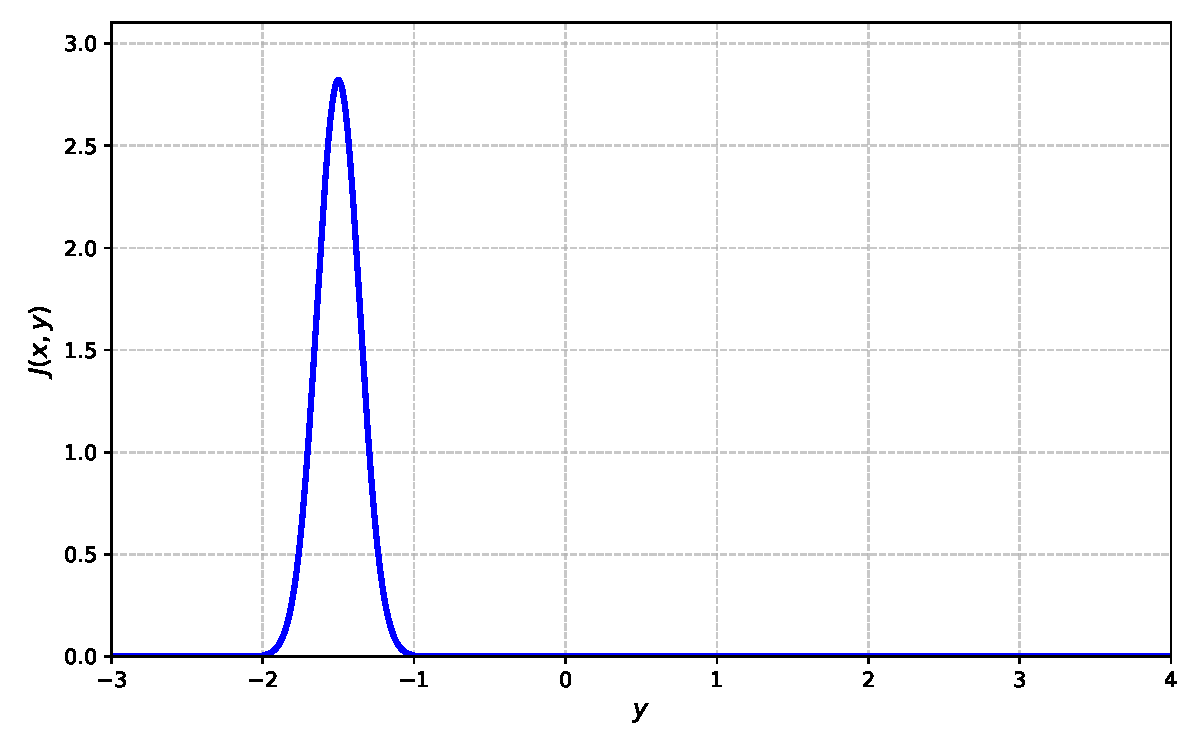
\includegraphics[width=0.5\linewidth]{Figures/时谐电流源J.pdf}
	    \caption{图名\label{图名}}
    \end{figure}
\end{frame}

\begin{frame}{多个子图(以1×2子图为例)}
    \begin{figure}[H]
        \centering
        % 第一行
        \begin{subfigure}[b]{0.45\textwidth}%[b]表示这一行所有子图的底部边缘(通常是子图标题的最后一行水平基线)对齐在同一条水平线上。这是学术排版中最常用、看起来最整齐的设置。
            \centering
            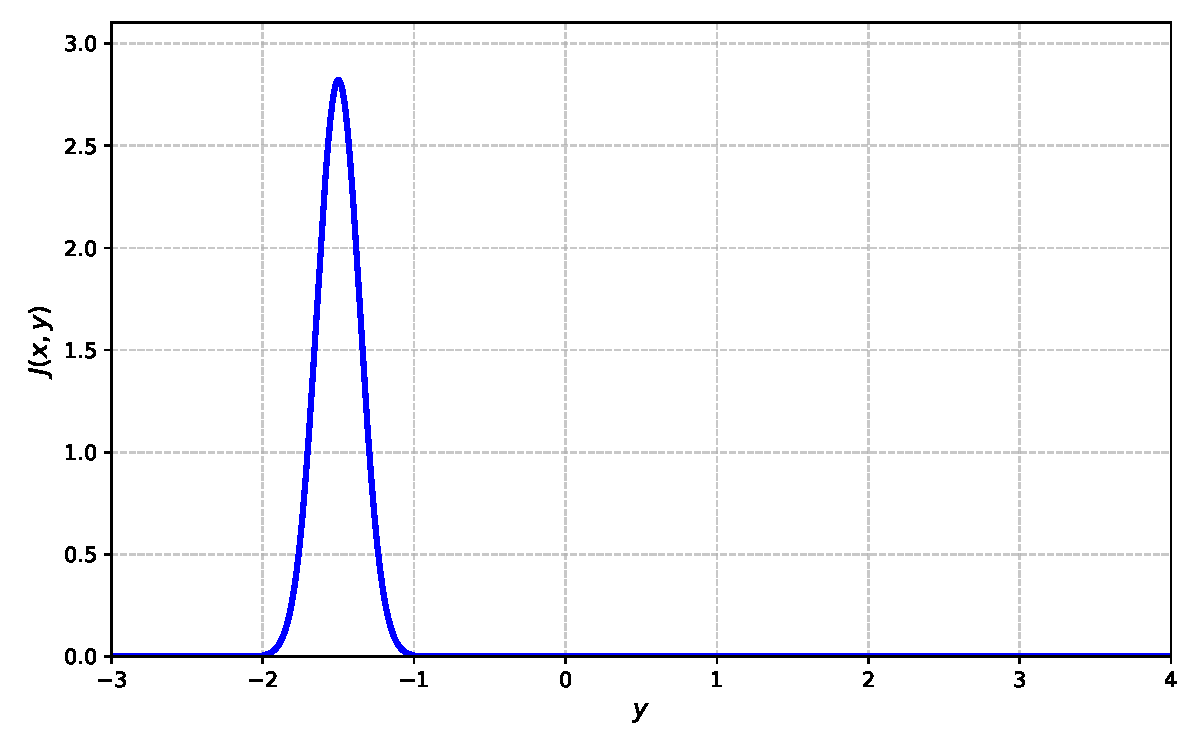
\includegraphics[width=\textwidth]{Figures/时谐电流源J.pdf}
            \caption{SubFigure1}
            \label{fig:sub1}
        \end{subfigure}
        \hfill % 使用 hfill 自动推开间距，比手动 hspace 更好控制
        \begin{subfigure}[b]{0.45\textwidth}
            \centering
            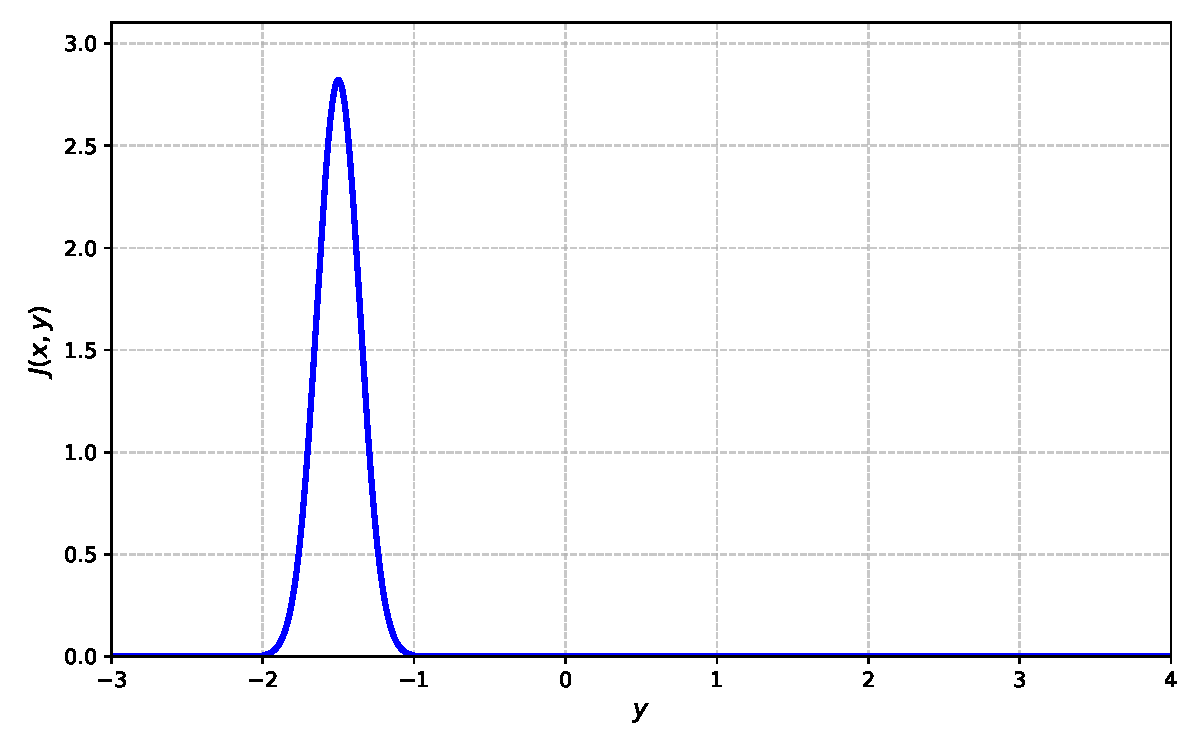
\includegraphics[width=\textwidth]{Figures/时谐电流源J.pdf}
            \caption{SubFigure2}
            \label{fig:sub2}
        \end{subfigure}
    
        \caption{1×2布局\label{fig:main}}
    \end{figure}
\end{frame}

% ---------------- 第三部分 ----------------
\section{引用测试}

\begin{frame}{交叉引用测试}
    单个子图\ref{图名}

    多个子图\ref{fig:main}
\end{frame}

\begin{frame}{参考文献引用测试}
  引用1\cite{ref1}

  引用2\cite{ref2}
\end{frame}

% ---------------- 参考文献 ----------------
\section*{参考文献}
% allowframebreaks 参数允许当参考文献过多时，自动换页
\begin{frame}[allowframebreaks]{参考文献}
  % 这里只需一句话，biblatex 会自动提取 ref.bib 中的文献并排版
  \printbibliography
\end{frame}

% ---------------- 结尾页 ----------------
\section*{致谢}
\begin{frame}
  \begin{center}
    {\Huge Thanks} \\
  \end{center}
\end{frame}

\end{document}